
\documentclass{llncs}
%
\usepackage{makeidx}  % allows for index generation
\usepackage{epsfig}
%
\title{Graph Neural Networks for 3D Bravais Lattices Classification}
\author{Aleksy Barcz \and Stanis{\l}aw Jankowski}
\institute{Warsaw University of Technology, Institute of Electronic Systems, Warsaw, Poland}
\begin{document}
\maketitle
%
\begin{abstract}
This paper presents the~computational capabilities of Graph Neural Networks in application to 3D crystal structures. The~Graph Neural Network model is described in terms of encoding and unfolded network. Results of classifying selected 3D Bravais lattices are presented.
\end{abstract}

\section{Introduction}
In the~domain of classification and regression we can distinguish two types of data. The~first type is the~standard, \emph{vectorial} data. Such data can be represented as vectors of a~constant length. Each position in such a~vector corresponds to a~numerical \emph{feature}. Each sample belonging to such data can be described by a~vector of features, ordered consistently among the~whole dataset. The~second type of data is the~\emph{structured} or \emph{graph} data. Each sample belonging to such data can be described by a~\emph{graph}, consisting of \emph{nodes} and \emph{edges}. Each node or edge can be described by its \emph{label}, which is a~constant-length vector of ordered numerical features. However, the~explicit information about each sample is stored not only in the~node and edge labels, but also in the~\emph{structure} of the~graph.

The~first attempts to process graph data with neural networks models were the~Hopfield networks, mapping from one graph node to adjacent nodes~\cite{goulon2005hopfield}. Subsequently, \emph{encoder-decoder} models were invented, like the~RAAM~\cite{pollack1990recursive} and LRAAM model~\cite{sperduti1994labelling}. A single RAAM/LRAAM model usually consists of two fully-connected three layer neural networks (inputs performing no computation, a~hidden layer and an output layer). The~first network, called the~\emph{encoder} is used to build a~lossless compressed representation of graph nodes, while the~\emph{decoder} network is used to restore the~original graph node representation from the~compressed code. Such models can be used to build a~compact representation of DPAGs (directed positional acyclic graphs), where the~representation of a~graph root node is treated as the~whole graph representation. Such a~representation can then be fed to a~standard feed-forward neural network for classification/regression purposes. Later on, the~Backpropagation Through Structure (BPTS) algorithm was formulated~\cite{goller1996learning}, addressing the~\emph{moving target} problem and introducing the~idea of the~\emph{unfolded network}. Finally, two models were created to process graph data without creating a~lossless encoding: the~Graph Machines~\cite{goulon2005learning} and the~Graph Neural Networks~\cite{scarselli2009graph}. Both models are designed to learn an encoding of graphs which is sufficient for a~graph classification/regression task. Such an approach proved to work well in various domains. Graph Machines were successfully used in many QSAR and QSPR tasks~\cite{goulon2007predicting}~\cite{goulon2011novel}, including most recently prediction of fuel compounds properties~\cite{saldana2013rational}. Graph Neural Networks were used in XML document mining~\cite{yong2006xml}, web page ranking~\cite{scarselli2005graph}, spam detection~\cite{scarselli2013solving}, object localisation in images~\cite{monfardini2006graph} and in image classification~\cite{quek2011structural}.

In the~field of material technology, the~properties of a~material often depend on defects in its crystal structure. Such defects may consist of a~vacant site in the~crystal lattice or of a~\emph{basis} substitution.
This article describes how three dimensional crystal structures, such as Bravais lattices, can be processed using Graph Neural Networks. By using a~graph oriented model, the~spacial location of lattice points can be described. By using node labels corresponding to lattice points, information about the~basis can be taken into account.


\section{The~Graph Neural Network Model}
The~Graph Neural Network model is a~connectionist model, capable of performing classification and regression on almost all types of graphs\cite{scarselli2009graph}. In particular, cyclic and acyclic, positional and non-positional, directed and undirected graphs can be processed by this model. A similar solution was the~recursive neural network model~\cite{bianchini2005recursive}. However, it is the~GNN that combined several existing techniques with a~novel training algorithm to produce a~very flexible graph processing model.

\subsection{Data}
A single GNN model is built for a~set of graphs (the~dataset). Each graph belonging to the~dataset can have a~different structure. The~whole dataset can be thus represented as a~single disconnected graph. Each $n$th graph node is represented by its label $\vec{l}_n$ of constant size $|\vec{l}_n| \geq 1$. Each directed edge $u \Rightarrow n$ (from $u$th to $n$th node) is represented by edge label $\vec{l}_{(n,u)}$ of constant size $|\vec{l}_{(n,u)}| \geq 0$. The~edge label size may differ from the~node label size. In the~implemented model undirected edges were represented as pairs of directed edges to account for the~mutual impact of connected nodes. For each $n$th graph node an output $\vec{o}_n$ of constant size can be sought - we say it's a~\emph{node-oriented} task. Alternatively, a~single output $\vec{o}_g$ can be sought for the~whole graph - in such case we say it's a~\emph{graph-oriented} task. In this paper a~node-oriented approach was chosen, as a~potentially more flexible one.

\subsection{Computation Units}
The GNN model consists of two computational units: the~transition unit $f_{\vec{w}}$ and the~output unit $g_{\vec{w}}$. The~vector of parameters $\vec{w}$ is distinct for each unit, however, for consistency with previous publications it will be denoted by $\vec{w}$ for both units. The~transition unit is used to build the~encoded representation of each node, $\vec{x}_n$ (the~\emph{state} of $n$th node). The~output unit is used to calculate the~output $\vec{o}_n$ for each node. Let's denote by $ne[n]$ the~set of neighbors of the~$n$th node, that is such nodes $u$ that are connected to the~$n$th node with a~directed edge $u \Rightarrow n$. Let's further denote by $co[n]$ the~set of directed edges from $ne[n]$ to the~$n$th node. For this implementation the~following transition and output functions were used:

\begin{equation}
\vec{x}_n = f_{\vec{w}}(\vec{l}_n, \; \vec{l}_{co[n]}, \; \vec{x}_{ne[n]}) \enspace ,
\label{eq:gnn_fmin}
\end{equation}

\begin{equation}
\vec{o}_n = g_{\vec{w}}(\vec{x}_n) \enspace .
\label{eq:gnn_gmin}
\end{equation}

The~GNN model offers two forms of the~$f_{\vec{w}}$ function, one better suited for positional graphs, the~other one for non-positional graphs. To make processing non-positional graphs possible, the~\emph{non-positional form} of $f_{\vec{w}}$ was chosen~\cite{scarselli2009graph}, which can be described as a~simple sum of $h_{\vec{w}}$ unit outputs. This yields the~final set of equations describing the~model:

\begin{equation}
\vec{x}_n = \sum_{u \in ne[n]}h_{\vec{w}}(\vec{l}_n, \; \vec{l}_{(n,u)}, \; \vec{x}_{u}) \enspace ,
\label{eq:gnn_ffinal}
\end{equation}

\begin{equation}
\vec{o}_n = g_{\vec{w}}(\vec{x}_n) \enspace .
\label{eq:gnn_gfinal}
\end{equation}

The~$h_{\vec{w}}$ and $g_{\vec{w}}$ units were implemented as fully-connected three layer neural networks. Hidden layers consisted for both networks of $tanh$ neurons. The~output layer of the~$h_{\vec{w}}$ network consisted of $tanh$ neurons, as the~state $\vec{x}_n$ must consist of bounded values only. The~output layer of the~$g_{\vec{w}}$ network consisted of neurons with linear activation function. During initialization, weights of both networks were set so that the~input to every $j$th neuron, $net_j$, was bounded assuming normalised input: $net_j \in (-1, 1)$. The~initial input weights corresponding to the state inputs were divided by an additional factor, i.e. the~maximum node indegree, to take into consideration the~fact, that the~state consists of a~sum of $h_{\vec{w}}$ outputs. All the~input data (node and edge labels) was normalised before feeding to the~model. The~$f_{\vec{w}}$ and $g_{\vec{w}}$ functions are presented in Fig.~\ref{fig:gnn_fg} altogether with one of the~corresponding edges, where the~comma-separated list of inputs stands for a~vector obtained by stacking all the~listed values one after another.

\begin{figure}[h!]
\begin{center}
	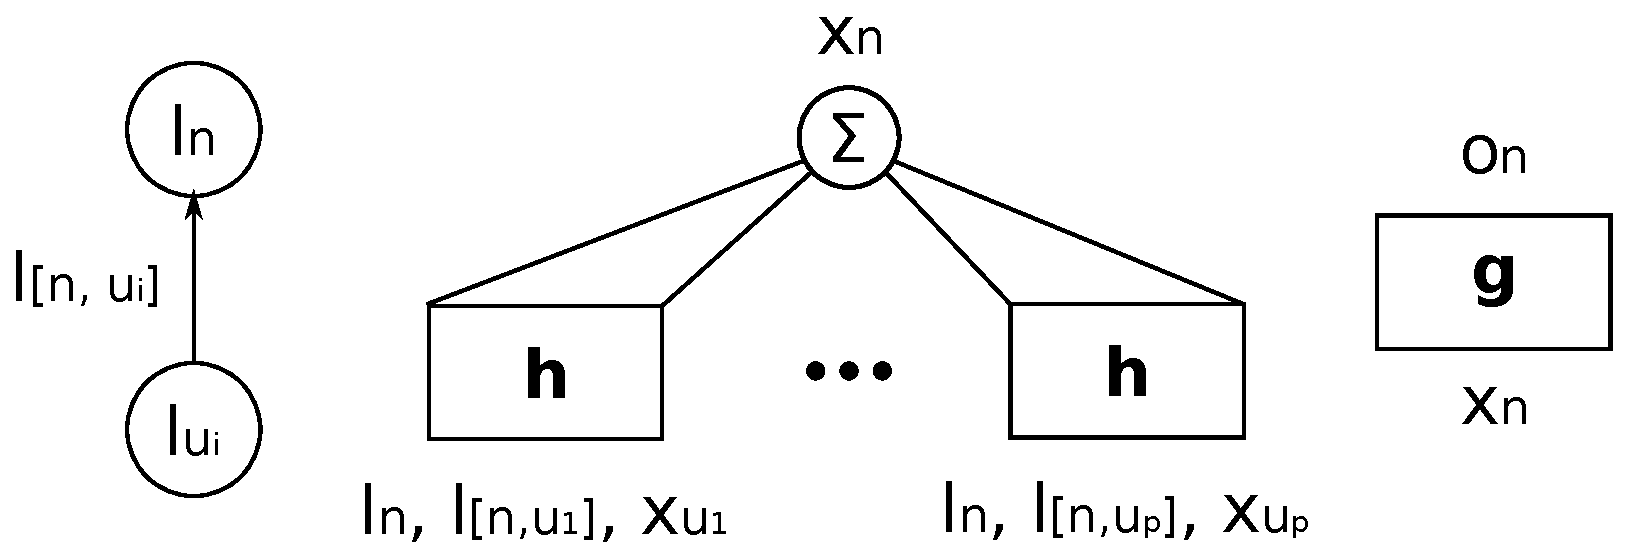
\epsfig{file=eps/f_ext2,width=11cm}
	\caption[]{The~$f_{\vec{w}}$ and  $g_{\vec{w}}$ functions for a~single node and one of the~corresponding edges}
	\label{fig:gnn_fg}
\end{center}
\end{figure}


\subsection{Encoding Network}
Graph processing by a~GNN model consists of two steps. The first step is to calculate the~state $\vec{x}_n$ for all nodes, using the~transition function $f_{\vec{w}}$ and exploiting the graph structure. The second step is to process this representation using the~output function $g_{\vec{w}}$. The~values of node states depend on one another, according to the~graph structure, so the~whole model can be described in terms of an \emph{encoding network}. The~encoding network consists of the $f_{\vec{w}}$ unit instances connected according to the~graph structure, with an instance of $g_{\vec{w}}$ unit connected at each node. It is important to remember, that there exists only one $h_{\vec{w}}$ and only one $g_{\vec{w}}$ network for the whole GNN. All the~instances are just copies of these two networks, using the~same sets of weights (the~\emph{shared weights} technique). A sample graph and the~corresponding encoding network are presented in Fig.~\ref{fig:gnn_encoding}. It can be seen that if a~graph contains cycles, the~state calculation must be an iterative process, to take into account all the~node dependencies. Furthermore, we would expect a~convergence to be reached, which is also addressed by the~GNN model.

\begin{figure}[h!]
\begin{center}
	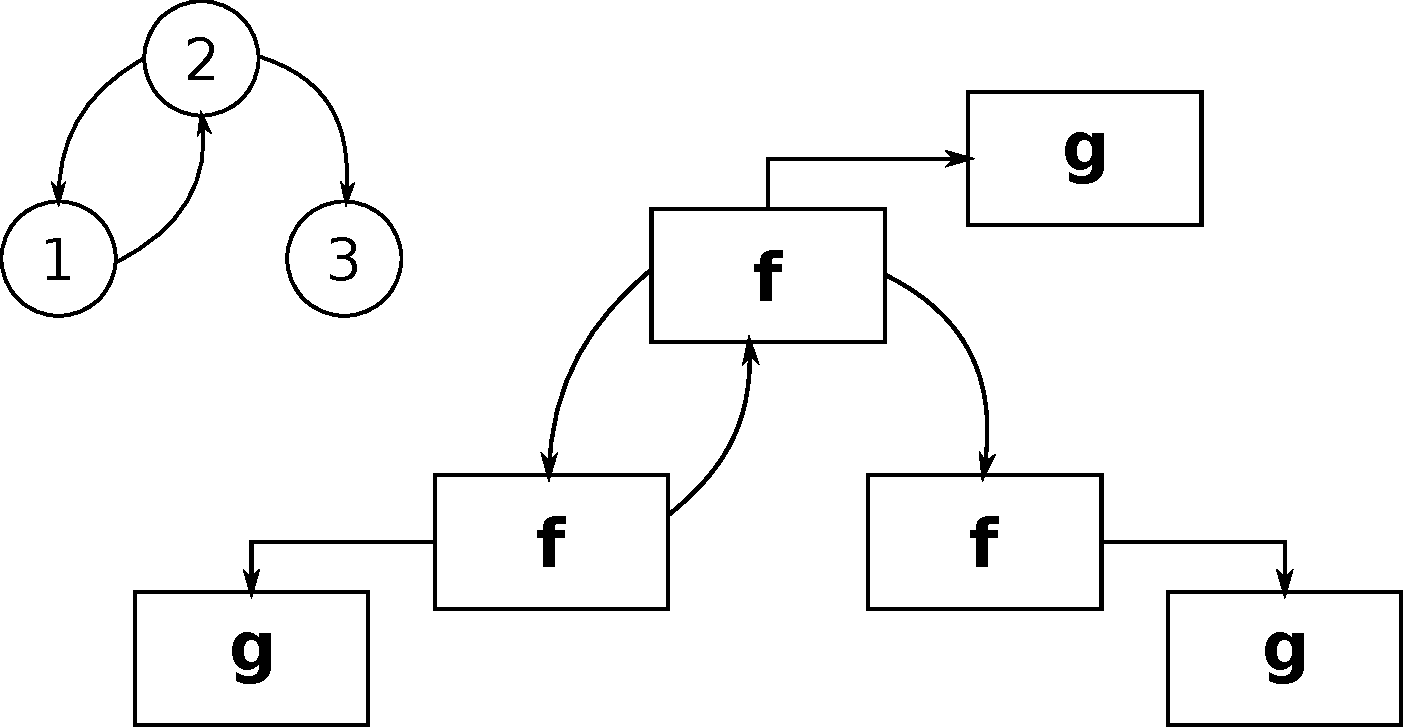
\epsfig{file=eps/encodinginc,width=8cm}
	\caption[]{A sample graph and the~corresponding encoding network}
	\label{fig:gnn_encoding}
\end{center}
\end{figure}


\subsection{Unfolding and Convergence}
To take into account all graph edges (which may form cycles), another representation of the~encoding network is used. The~encoding network is virtually \emph{unfolded} in time in such a~way, that at each time step $t_i$ all $f_{\vec{w}}$ units are taken into consideration and the~connections between them exist only between subsequent time steps. In such a~way all cycles can be processed naturally without additional effort. Let's define the~\emph{global state} $\vec{x}$ as the~set of all node states. Let's define $\vec{l}$ as the~set of all node and edge labels. Let's further define $\vec{o}$ as the~set of all node outputs. The~\emph{global transition function} $F_{\vec{w}}$ and \emph{global output function} $G_{\vec{w}}$, being the~unfolded network counterparts of $f_{\vec{w}}$ and $g_{\vec{w}}$, are defined as follows:

\begin{equation}
\vec{x} = F_{\vec{w}}(\vec{l}, \; \vec{x}) \enspace ,
\label{eq:gnn_fglobal}
\end{equation}

\begin{equation}
\vec{o} = G_{\vec{w}}(\vec{x}) \enspace .
\label{eq:gnn_gglobal}
\end{equation}

The~global state $\vec{x}$ is computed at each time step and is expected to converge to $\hat{\vec{x}}$ after a~finite number of steps. Then, the~output $\vec{o}_n$ is calculated by the~$g_{\vec{w}}$ units. The~output error $\vec{e}_n = (\vec{d}_n - \vec{o}_n)^2$ (where $\vec{d}_n$ stands for the~expected output) is calculated and backpropagated through the~output units, yielding $\frac{\partial e_{\vec{w}}}{\partial \vec{o}}\cdot \frac{\partial G_{\vec{w}}}{\partial \vec{x}}(\hat{\vec{x}})$. That value is backpropagated through the~unfolded network using the~BPTT/BPTS algorithm. Additionally, at each time step the~$\frac{\partial \vec{e}_{\vec{w}}}{\partial \vec{o}}\cdot \frac{\partial G_{\vec{w}}}{\partial \vec{x}}(\hat{\vec{x}})$ error is injected to the~$f_{\vec{w}}$ layer. In such a~way the~error backpropagated through the~$f_{\vec{w}}$ layer at time $t_i$ comes from two sources. Firstly, it is the~original output error of the~network $\frac{\partial \vec{e}_{\vec{w}}}{\partial \vec{o}}\cdot \frac{\partial G_{\vec{w}}}{\partial \vec{x}}(\hat{\vec{x}})$. Secondly, it is the~error backpropagated from the~subsequent time layers of the~$f_{\vec{w}}$ unit from all nodes connected with the~given node $u$ by an edge $u \Rightarrow n$. The~backpropagation continues until the~error value converges, which usually take less time steps than the~state convergence. The~unfolding and error backpropagation phases are presented in Fig.~\ref{fig:gnn_forback}.

\begin{figure}[h!]
\begin{center}
	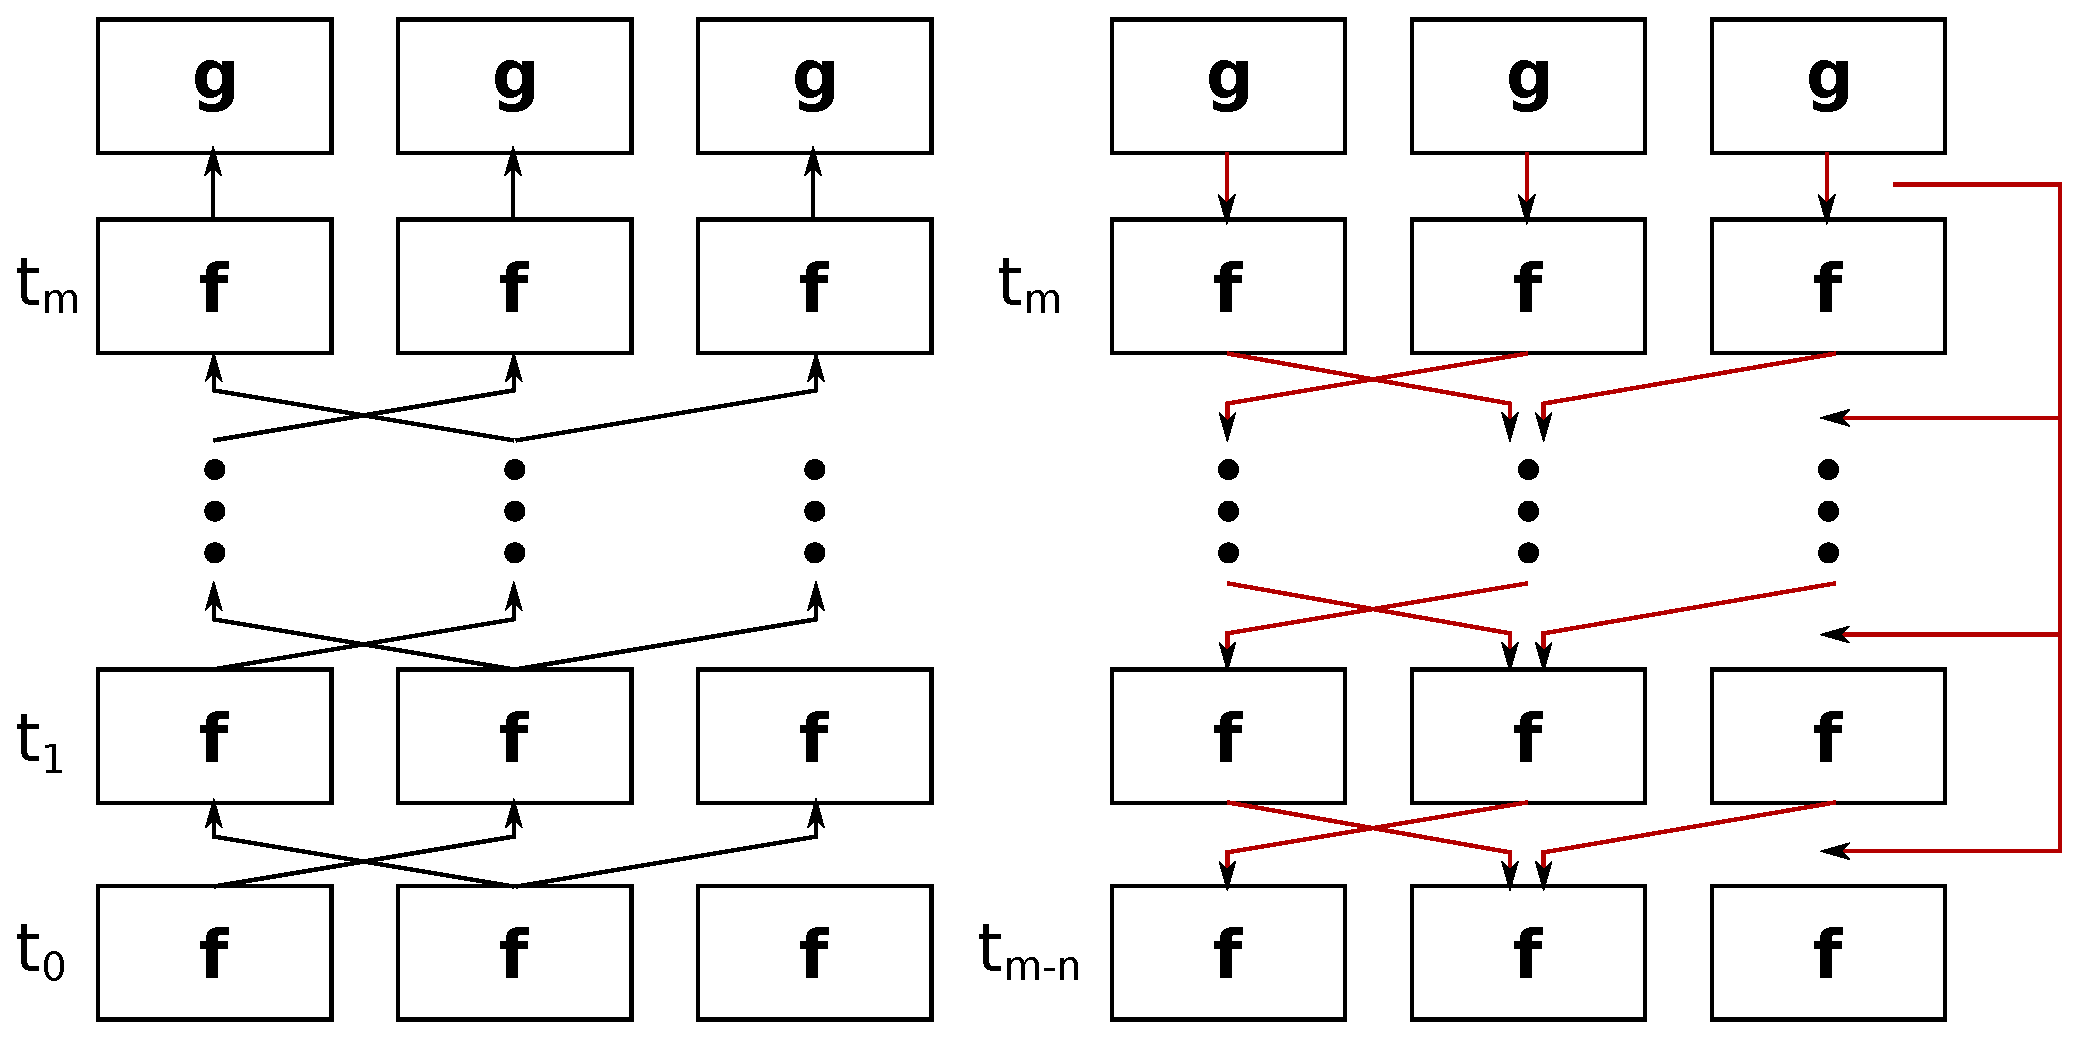
\epsfig{file=eps/forback2,width=11.5cm}
	\caption[]{Unfolded encoding network for the~sample graph and backpropagation}
	\label{fig:gnn_forback}
\end{center}
\end{figure}

The~described algorithm makes one important assumption: we want the~global state $\vec{x}$ to converge. To assure convergence, $F_{\vec{w}}$ must be a~\emph{contraction map}. According to Banach Theorem, this guarantees that the~state calculation will converge to a~unique point $\hat{\vec{x}}$ and the~convergence will be exponentially fast. To assure the~contraction property, a~penalty term $\frac{\partial p_{w}}{\partial w}$ is added to the~total $\frac{\partial e_{h_w}}{\partial w}$ error term after performing BPTS. The penalty value $p_{\vec{w}}$ is calculated as follows.
Let $\vec{A} = \frac{\partial F_{\vec{w}}}{\partial \vec{x}}(\vec{x}, \; \vec{l})$ be a block matrix of size $N \times N$ with blocks of size $s \times s$, where $N$ is the number of nodes in the processed graph and $|\vec{x}_n| = s$ is the state size for a single node. A single block $\vec{A}_{n,u}$ measures the influence of the $u$th node on the $n$th node if an edge $u \Rightarrow n$ exists or is zeroed otherwise. Let's denote by $I_u^j$ the influence of $u$th node on the $j$th element of state $\vec{x}_n$ (Eq.~\ref{eq:gnn_pw_inf}). The penalty $p_{\vec{w}}$ added to the network error $e_{\vec{w}}$ is defined by Eq.~\ref{eq:gnn_pw}.

\begin{equation}
p_{\vec{w}} = \sum_{u \in N} \sum_{j = 1}^{s} L(I_u^j, \; \mu) \enspace ,
\label{eq:gnn_pw}
\end{equation}

\begin{equation}
L(y, \; \mu) = \left\{
\begin{array}{l l}
	y - \mu		& \quad \mbox{if} \enspace y > \mu \\
	0			& \quad \mbox{otherwise}
\end{array} \right. \enspace ,
\label{eq:gnn_pw_L}
\end{equation}

\begin{equation}
I_u^j =  \sum_{(n, u)} \sum_{i = 1}^{s} |\vec{A}_{n, u}^{i, j}| \enspace .
\label{eq:gnn_pw_inf}
\end{equation}


This does not guarantee that $F_{\vec{w}}$ will remain a~contraction map, as the~penalty is added post factum and it must be tuned using the~contraction constant $\mu$. However, even if the~convergence isn't always reached, the~model can still be trained and yield good results. The~necessary constraint in such cases is a~maximum number of unfolding and error backpropagation steps.


\section{Bravais Lattices}
In crystallography, a~crystal structure can be described by a~\emph{lattice} and a~\emph{basis}~\cite{kittel1986introduction}. The~lattice describes the~location of lattice points in space, while the~basis is a~group of atoms (or a~single atom) that is placed at each lattice point. A sample lattice, a basis and the resulting two dimensional crystal structure are presented in Fig.~\ref{fig:lattice}. A Bravais lattice in three dimensional space is an infinite array of discrete points, generated by translation operations $T$:

\begin{equation}
T = n_1a + n_2b + n_3c \enspace .
\end{equation}

Each translation is described by three constant parameters: $a$, $b$ and $c$ which are called the~\emph{primitive vectors} and three integers: $n_1$, $n_2$ and $n_3$. If we translate the~lattice by any such vector $T$, we will obtain the~same lattice. A parallelepiped formed from the~primitive vectors is called a~\emph{primitive cell}. A primitive cell is a~basic component of a~crystal structure. We can distinguish 14 Bravais lattices in three dimensions, differing in the~primitive vectors length relations, the~angles between them and the~presence of additional lattice points in the~cell.


\begin{figure}[h!]
\begin{center}
	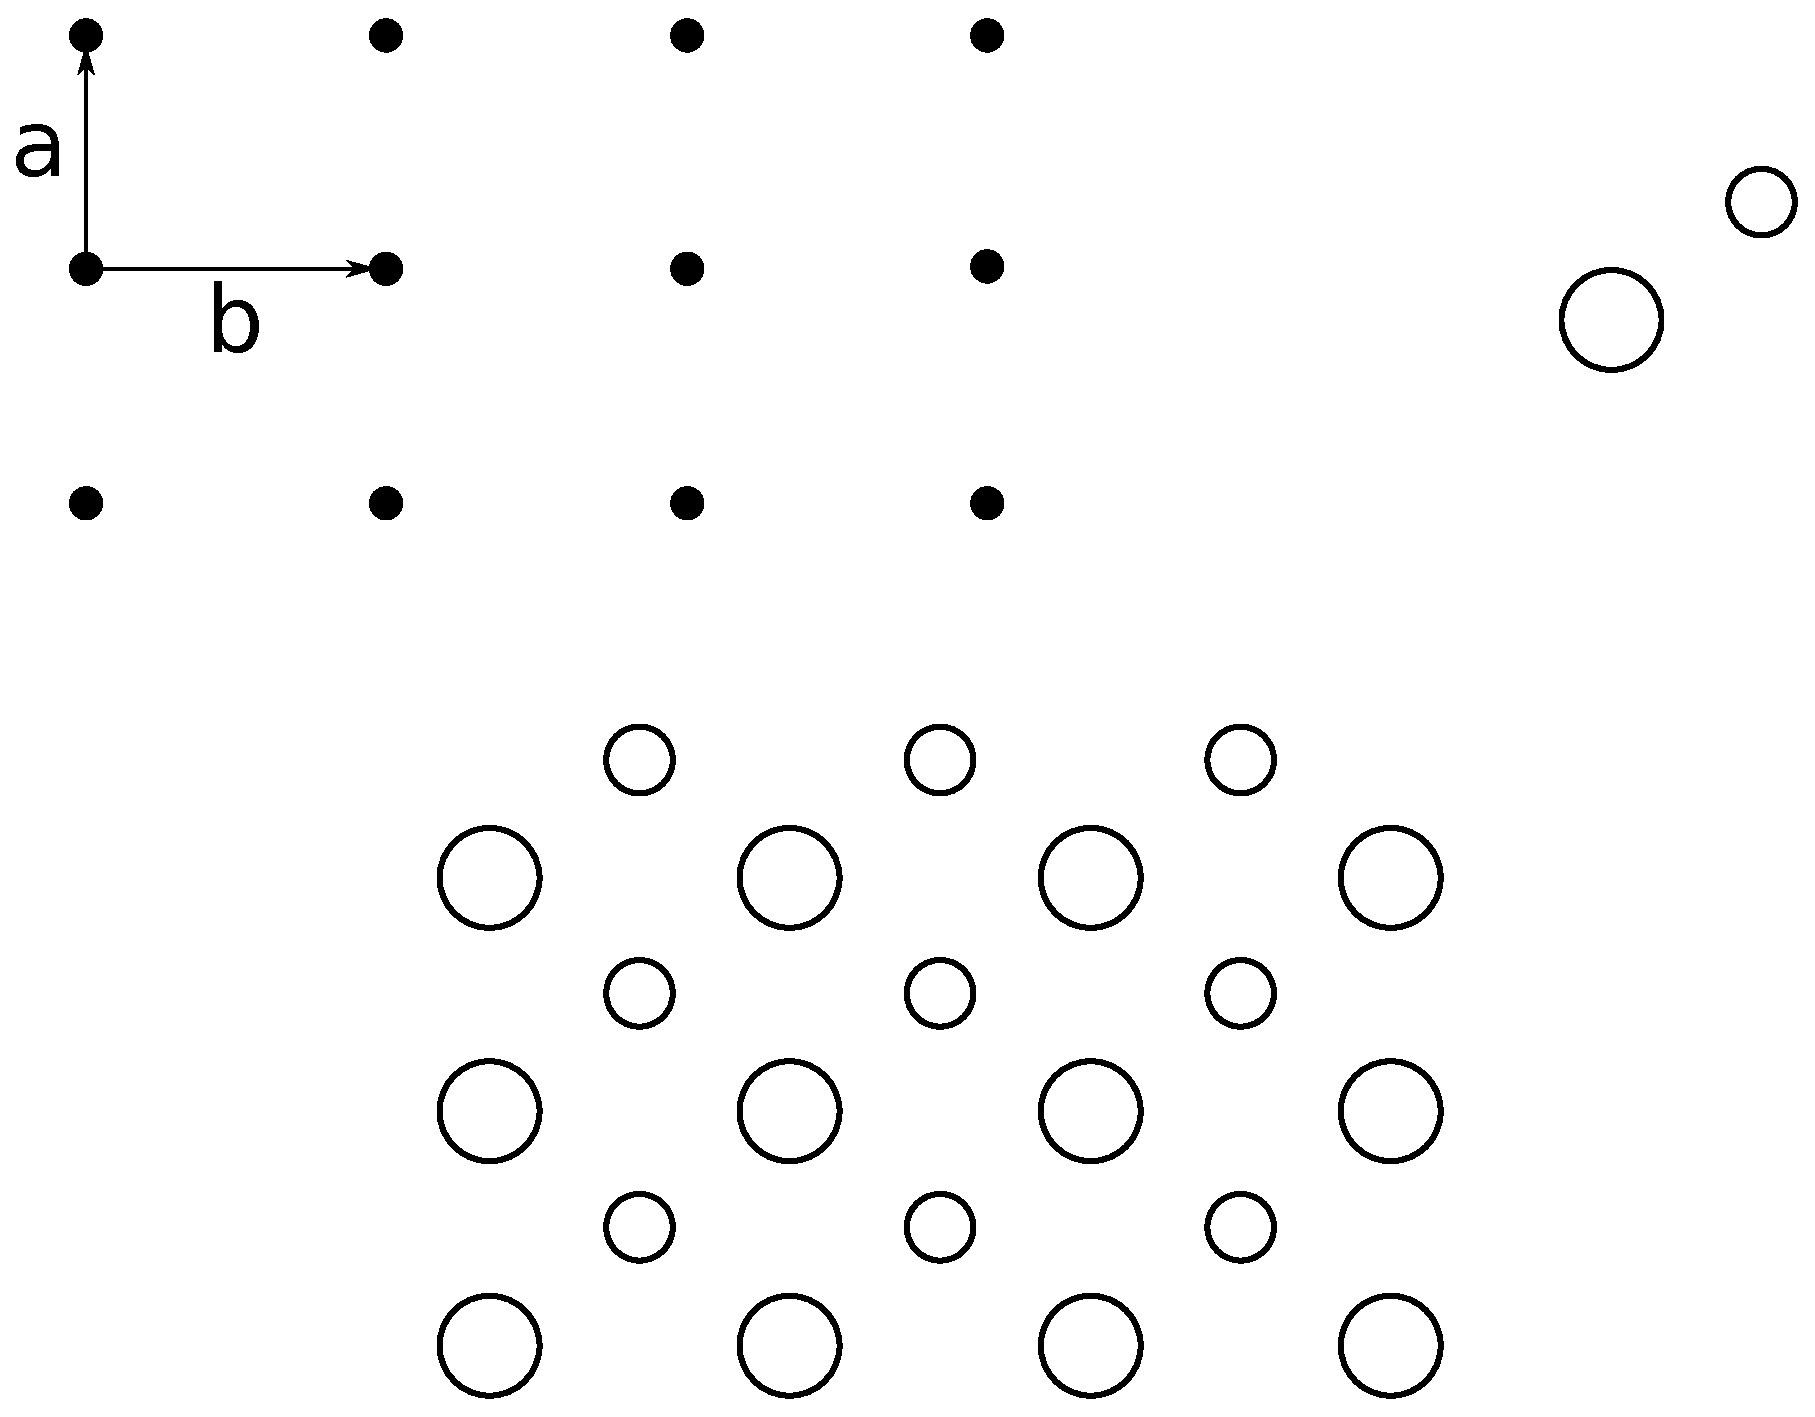
\epsfig{file=eps/lattice,width=6cm}
	\caption[]{A sample lattice, a basis and the resulting crystal structure}
	\label{fig:lattice}
\end{center}
\end{figure}


Many material properties depend on crystal structure defects, which are introduced on purpose. A defect may e.g. consist of an atom missing at one of the~lattice points (vacancy) or of a~different atom introduced at one of the~lattice points (substitution). Properties of materials containing a~particular defect are determined experimentally by producing a~specimen and testing it in a~laboratory. Modelling of such phenomena with neural network models could prove useful for approximating these properties before the~actual experiments take place.

\section{Experimental Results}
For the~scope of this work, two simple Bravais lattices were chosen for experiments: the~primitive (P) tetragonal lattice and the~body-centered (I) tetragonal lattice, containing additional lattice point in the~center of each cell. For both tetragonal lattices $a = b \neq c$, as presented in Fig.~\ref{fig:bravais}. For all the~experiments each crystal structure was represented by a~single cell. Each lattice point was described as a~graph node, with node label containing information about the~basis used at this node. The~mutual location of two adjacent points $u$ and $n$ was described as a~pair of directed edges, each containing in its label the~3D cartesian coordinates of the~vector $u \Rightarrow n$ or $n \Rightarrow u$, respectively. In such way, the~description of a~cell was independent from the~actual location of the~cell in space, which was the~goal. A spherical coordinates system was also tried out, yielding similar results to the~cartesian one.


\begin{figure}[h!]
\begin{center}
	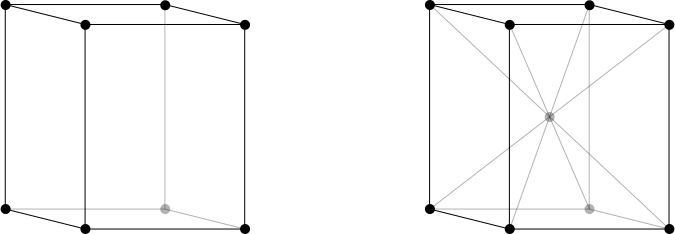
\epsfig{file=eps/tetragonal,width=7cm}
	\caption[]{Simple tetragonal cell (P) and body-centered tetragonal cell (I)}
	\label{fig:bravais}
\end{center}
\end{figure}


For every experiment the~dataset was generated as follows. First a~single graph (cell) was created as a~cubic (P) cell $a = b = c = 1$. Node labels were set to $1$ ($|l_n| = 1$, $l_n = 1$), unless stated otherwise. A second graph, cubic (I) cell, was created by introducing an additional node in the~center of the~graph. Then, datasets were generated by random scaling of all the~input graphs edges using factors pertaining to uniform distribution $U(-5, 5)$, but maintaining the~tetragonal constraint: $a = b \neq c$. Then, a~small random error $\varepsilon$ with zero mean and standard deviation equal to $0.01$ was added to all node and edge labels. For every experiment the~dataset consisted of two classes of 200 graphs each. Among each class every graph node had its expected output set to the~same value: $1$ or $-1$, depending on the~class. During evaluation, a~node was assigned to class depending on the~sign of its output $o_n$. For every experiment, the~training set consisted of 50 graphs, while the~test set consisted of 150 graphs.

For every experiment, the~state size $|\vec{x}_n|$ was set to $5$. The~number of hidden neurons was set for both networks to $5$. For the~output network linear neurons were used as output neurons. The~contraction constant $\mu$ was set to $30$ as smaller values tended to disturb the~learning process significantly. The~maximum number of state calculation and error backpropagation steps was set to $200$. The~number of full training iterations (forward-backward) was set to $200$, as it could be seen that for some GNNs the~RMSE on training set began to drop significantly only after more than $100$ iterations. In each experiment the~best GNN was selected as the~one that achieved the~smallest RMSE on the~training set. Then, the~selected GNN was evaluated on the~test set. The~training set for each experiment consisted of $50$ samples from each of the~two classes ($100$ samples in total). The~test set consisted of $150$ samples from each class ($300$ samples in total).

\subsection{Structural Difference}
For this experiment, a~tetragonal (P) dataset was compared to a~tetragonal (I) dataset. All node labels were set to the~same value. Thus, the~task to solve was to distinguish cells with the~central atom missing from full tetragonal (I) cells. The~results achieved by the~selected GNN are presented in Table~\ref{tab:struct}. It can be seen, that a~GNN can be trained to deal very well with such a~task, in which the~number of nodes in two graphs differs.

\begin{table}[h!]
\begin{center}
\caption{Structural difference - results}
\begin{tabular}{llll}
\hline\noalign{\smallskip}
 & accuracy & precision & recall\\
\noalign{\smallskip}
\hline
\noalign{\smallskip}
training set & 98.94\% &  98.51\% & 99.25\% \\
test set & 98.82\% & 98.03\% &  99.50\% \\
\hline
\label{tab:struct}
\end{tabular}
\end{center}
\end{table}


\subsection{Single Substitution}
For this experiment, two tetragonal (I) datasets were used. In one dataset all node labels were set to $1$, while in the~other one the~labels of central nodes were set to $2$, to simulate a~single atom substitution. The~unusually good results for the small random error, presented in Table~\ref{tab:subst}, can be explained by the~simplicity of the~task. As node labels are explicitly given to the~model (not alike the~structure of the~graph, which was the~case described in the~previous section), a~simple linear classifier would be sufficient for this task, even taking into consideration the~noise applied. To check the model performance with a more demanding task, a larger random error $\varepsilon$ with zero mean and standard deviation equal to $0.1$ was added to the original node and edge labels and a new classifier was trained. The results are significantly worse, however, it must be stated, that such a random error disturbs greatly the graph structure in the case of small edge lengths.

\begin{table}[h!]
\begin{center}
\caption{Single substitution - results}
\begin{tabular}{llll}
\hline\noalign{\smallskip}
 & accuracy & precision & recall\\
\noalign{\smallskip}
\hline
\noalign{\smallskip}
training set ($sd \enspace \varepsilon = 0.01$) & 100\% &  100\% & 100\% \\
test set ($sd \enspace \varepsilon = 0.01$) & 100\% & 100\% & 100\% \\
training set ($sd \enspace \varepsilon = 0.1$) & 96.00\% &  96.00\% & 96.00\% \\
test set ($sd \enspace \varepsilon = 0.1$) & 94.92\% & 95.29\% & 94.51\% \\
\hline
\label{tab:subst}
\end{tabular}
\end{center}
\end{table}

\subsection{Substitution Location Difference}
For this experiment, two tetragonal (I) datasets were used, both of them containing a~single substitution (node label of one node set to $2$). However, for the~first set the~substituted node was the~central node, while for the~other set one of the~corner nodes was substituted. Therefore, every graph had eight nodes labelled as $1$ and a~single node labelled as $2$. The~location of the~substituted node was different for the~two sets and the~task was to find this difference basing on nodes connections. This task proved to be the~most difficult for the~GNN model. Not only the~difference in node labels was to be taken into consideration, but also the~different placement of the~substituted node, so the~structure of the~graph had to be exploited properly. Nevertheless, the~GNN model proved to achieve very good results in this task, as presented in Table~\ref{tab:substloc}.

\begin{table}[h!]
\begin{center}
\caption{Substitution location difference - results}
\begin{tabular}{llll}
\hline\noalign{\smallskip}
 & accuracy & precision & recall\\
\noalign{\smallskip}
\hline
\noalign{\smallskip}
training set & 96.33\% &  94.26\% & 98.66\% \\
test set & 95.07\% & 92.05\% & 98.66\% \\
\hline
\label{tab:substloc}
\end{tabular}
\end{center}
\end{table}

\section{Conclusion}
The~Graph Neural Network is a~model successfully used in many two dimensional graph processing tasks. This article presents the~capabilities of the~GNN model to process three dimensional data, such as crystal structures. The~main difference of this data lays in the~fact, that the~spatial location of all the~nodes must be taken into consideration and not only the~edge and node properties. The~tasks used for testing the~GNN model were selected so as to present how the~GNN can be used to deal with various structural and property differences. The~model proved to work well in all the~tasks, including a simulated crystal structure vacancy defect and two different atom substitution defects.

\bibliography{bib/crystal,bib/gnn}
\bibliographystyle{splncs}
\end{document}
